\section{Results}

\begin{figure}[t]
\centering
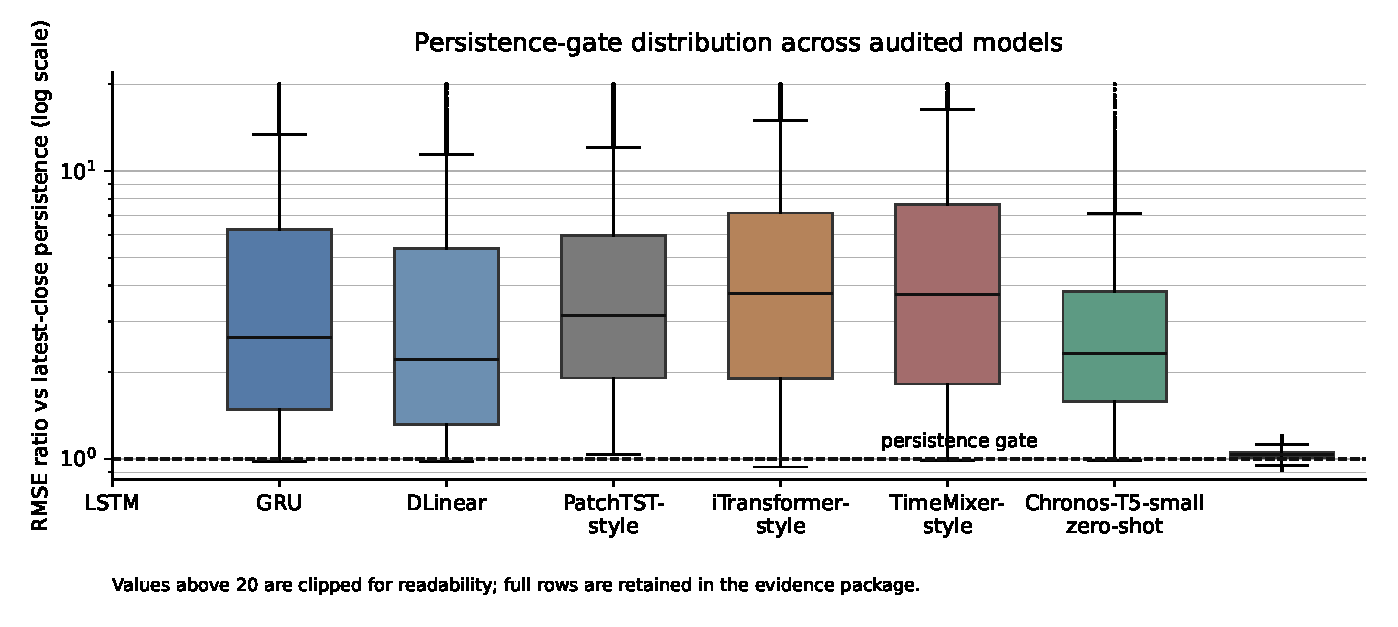
\includegraphics[width=0.92\textwidth]{figures/Figure1_RMSE_Ratio_Distribution.eps}
\caption{Distribution of RMSE ratios relative to latest-close persistence. Values below the dashed line beat persistence; values above it underperform. The supervised compact implementations are evaluated with full rolling-origin tests, while Chronos-T5-small uses the sampled-origin zero-shot protocol. Extreme ratios above 20 are clipped only for visualization.}
\label{fig:rmse_ratio_distribution}
\end{figure}

\subsection{Supervised Models Rarely Pass}

Table~\ref{tab:model_gate_summary} and Fig.~\ref{fig:rmse_ratio_distribution} show the central result. Across 35,640 supervised neural rows, only 23 pass the persistence gate. LSTM passes 8 of 5,940 rows, GRU passes 5, DLinear passes none, and the three scaled-down modern implementations pass only 10 rows combined. The median RMSE ratios are all far above 1.0, ranging from 2.221 for GRU to 3.766 for PatchTST-style. These are not small losses to persistence; they are systematic underperformance relative to a no-training baseline under this absolute-price protocol.

The horizon breakdown in Table~\ref{tab:horizon_summary} shows that longer horizons are somewhat easier, but the conclusion does not change. All supervised model groups have median RMSE ratios above 1.0 at 1-day, 5-day, and 10-day horizons. The 1-day case is especially severe because latest-close persistence is nearly aligned with the target.

\subsection{Chronos Has Local Wins But Not a Stable Advantage}

Chronos-T5-small is meaningfully different from the supervised models. It passes 133 of 990 sampled-origin rows. The nominal pass rate of 13.4\% exceeds that of the supervised models, but direct row-count comparisons are confounded because Chronos was evaluated on a sparse sampled-origin protocol rather than the full rolling-origin protocol used for the supervised models. Therefore, the more reliable aggregate statistic is the median RMSE ratio, which remains above 1.0. Its best cases include individual ETFs, U.S. stocks, and Hang Seng stocks where RMSE ratios fall below 0.95. This suggests that zero-shot foundation forecasters can sometimes improve on latest-close persistence.

However, the aggregate result remains negative. Chronos has median RMSE ratio 1.035 with a bootstrap 95\% confidence interval of [1.033, 1.037]. The one-sided Wilcoxon test strongly rejects equality in the direction of ratios above 1.0. Because the sampled origins may yield less stable tail estimates, the observed pass count should be interpreted as evidence that zero-shot forecasting can occasionally surpass persistence, not as evidence that Chronos-T5-small consistently outperforms the latest close. To verify that sparse origin sampling does not drive this interpretation, we also ran a full-origin Chronos subset covering two assets per dataset, both price modes, and all three horizons. In that 60-row verification, Chronos passed only 2 rows and had a median RMSE ratio of 1.028, consistent with the main sampled-origin conclusion.

\subsection{Cross-Market Pattern}

The underperformance is not confined to a single asset list. Supervised models fail to clear the persistence gate across U.S. large-cap equities, technology-heavy equities, Hong Kong large caps, and ETFs. Hang Seng assets produce more of the rare supervised passes, and ETFs produce the highest Chronos pass rate, but no dataset reverses the overall conclusion. The audit therefore supports a bounded cross-market claim: for price-level forecasting, compact learned forecasters and Chronos-T5-small do not automatically translate model sophistication into out-of-sample improvement over latest-close persistence.
